\begin{frame}
\frametitle{Backup 1: GPU Workload and design trade-off}
\begin{block}{Why GPUs Have High Memory bandwidth?}
Memory Bandwidth $\propto$ (Clock Rate $\times$ Memory Bus width)
\end{block}
\begin{block}{Why such design?}<2->
\begin{itemize}
\item<3-> CPU: Use \alert{Cache} to inmprove memory performance.
\item<4-> GPU Workload: 3D rendering, large dataset of polygons and textures, too large working set to fit in cache.
\item<5-> GPU: the only way -- wider memory bus + faster clock rate
\item<6-> Price( NVIDIA GTX 285 GPU with \alert{1 GB} memory ) \alert{$\approx$} Price ( Intel Core i7 CPU with \alert{6 GB} memory ).
\end{itemize}
\end{block}
\end{frame}

\begin{frame}
\frametitle{Backup 2: Performance Slowdown Over Native Implementations}
\begin{columns}
\column{0.50\textwidth}
\begin{block}{MarsCUDA vs CUDA. Slowdown $= T_{MarsCUDA}/T_{CUDA}$}
\includegraphics[width=1.0\linewidth]{figure/MarsGPU_CUDA.eps}
\end{block}
\column{0.50\textwidth}
\begin{block}{MarsCPU vs pthreads. Slowdown $= T_{MarsCPU}/T_{pthreads}$}
\includegraphics[width=1.0\linewidth]{figure/MarsCPU_pthread.eps}
\end{block}
\end{columns}
\end{frame}
